 \begin{center}
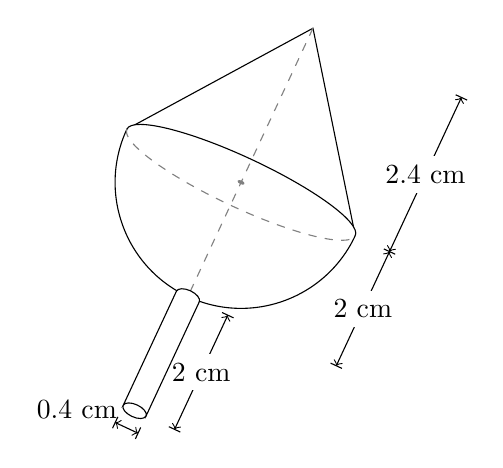
\begin{tikzpicture}[rotate=155,scale=0.8]
\draw(0,0)--(2,-2.7)--(4,0);
\draw[fill=white,draw=black](0,0)arc(180:360:2 and 0.4);
\draw(1.8,4)arc(180:0:.2 and .1);
\draw(0,0)arc(180:0:2);
\draw[fill=gray,draw=gray](1.95,0)arc(180:-180:.05 and .02);
\draw[dashed, gray](2,-2.7)--(2,2)(4,0)arc(0:180:2 and 0.4);
\draw[<->](1.3,2)--(1.3,4);
\draw(1.3,3)node[rectangle,fill=white]{$2$ cm}(1.2,2)--(1.4,2)(1.2,4)--(1.4,4);
\draw[fill=white,draw=black](1.8,2)arc(180:360:.2 and .1)--(2.2,4)arc(0:-180:.2 and .1)--cycle;
\draw[<->](-0.6,2)--(-0.6,0);
\draw(-0.6,1)node[rectangle,fill=white]{$2$ cm}(-0.7,0)--(-0.5,0)(-0.7,2)--(-0.5,2);
\draw[<->](-0.6,0)--(-0.6,-2.7);
\draw(-0.6,-1.35)node[rectangle,fill=white]{$2.4$ cm}(-0.7,-2.7)--(-0.5,-2.7);
\draw(2.2,4.2)--(2.2,4.4)(1.8,4.2)--(1.8,4.4);
\draw[<->](2.2,4.3)--(1.8,4.3);
\draw(2,4.3)node[anchor=south east]{$0.4$ cm};
\end{tikzpicture}\end{center}
\begin{center}Note: Diagram is not to scale. \end{center}
An aspiring fast food entrepreneur is designing a top for his first kid's meal toy.  The top is comprised of a cylindrical handle which connects to a hemisphere that shares its base with a right cone.  He plans to make the top using the dimensions as marked in the diagram.  His materials cost will be \$0.14 per cubic centimeter.  He wanted to make the tops solid until he discovered how much that would cost per toy, so instead he's hollowed out $80\%$ of the material from the design.  How much, in dollars, will it cost him to make each toy? \\\\


\ifsat
	\begin{enumerate}[label=\Alph*)]
	\end{enumerate}
\else
\fi

\ifacteven
	\begin{enumerate}[label=\textbf{\Alph*.},itemsep=\fill,align=left]
	\end{enumerate}
\else
\fi

\ifactodd
	\begin{enumerate}[label=\textbf{\Alph*.},itemsep=\fill,align=left]
	\end{enumerate}
\else
\fi

\ifgridin
$.758 $
\else
\fi

